\documentclass[tikz,border=12pt]{standalone}
\usepackage{amsmath,amssymb}
\usetikzlibrary{positioning,arrows,shapes,fit,calc,backgrounds,decorations.pathmorphing}
\begin{document}
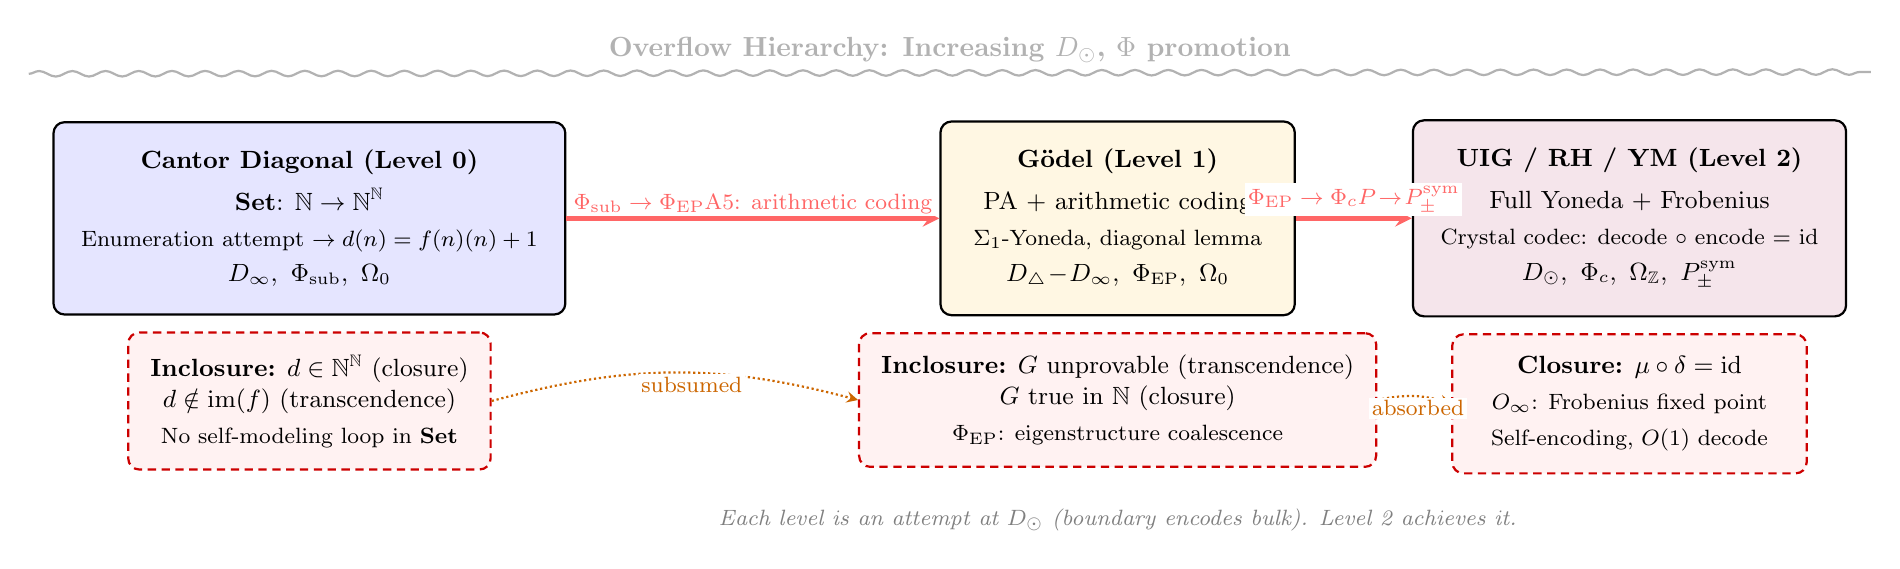
\begin{tikzpicture}[
  box/.style={rectangle,draw,thick,rounded corners,fill=#1!10,inner sep=10pt,align=center,minimum width=2.2cm,font=\small},
  arrow/.style={->,>=stealth,thick,blue!60},
  complabel/.style={font=\footnotesize,fill=white,inner sep=1pt},
  bigarrow/.style={->,>=stealth,ultra thick,red!60},
  inclosure/.style={rectangle,draw=red!80!black,thick,densely dashed,rounded corners,fill=red!5,inner sep=8pt,align=center,font=\small},
]

% === CANTOR LEVEL 0 ===
\node[box=blue,minimum width=4.5cm] (cantor) at (0,0) {
\textbf{Cantor Diagonal (Level 0)}\\[4pt]
$\mathbf{Set}$: $\mathbb{N} \to \mathbb{N}^{\mathbb{N}}$\\[2pt]
\footnotesize Enumeration attempt $\to d(n)=f(n)(n)+1$\\[2pt]
$D_\infty,\ \Phi_\text{sub},\ \Omega_0$
};

% The diagonal element
\node[inclosure,below=0.2cm of cantor,minimum width=4.5cm] (inc0) {
\textbf{Inclosure:} $d \in \mathbb{N}^{\mathbb{N}}$ (closure)\\
$d \notin \text{im}(f)$ (transcendence)\\[2pt]
\footnotesize No self-modeling loop in $\mathbf{Set}$
};

% === GODEL LEVEL 1 ===
\node[box=yellow!50!orange,right=2.0cm of cantor,minimum width=4.5cm] (godel) at (6,0) {
\textbf{G\"odel (Level 1)}\\[4pt]
PA + arithmetic coding\\[2pt]
\footnotesize $\Sigma_1$-Yoneda, diagonal lemma\\[2pt]
$D_\triangle\!-\!D_\infty,\ \Phi_\text{EP},\ \Omega_0$
};

\node[inclosure,below=0.2cm of godel,minimum width=4.5cm] (inc1) {
\textbf{Inclosure:} $G$ unprovable (transcendence)\\
$G$ true in $\mathbb{N}$ (closure)\\[2pt]
\footnotesize $\Phi_\text{EP}$: eigenstructure coalescence
};

% === GRAMMAR LEVEL 2 ===
\node[box=purple!80!black,right=2.0cm of godel,minimum width=4.5cm] (grammar) at (12,0) {
\textbf{UIG / RH / YM (Level 2)}\\[4pt]
Full Yoneda + Frobenius\\[2pt]
\footnotesize Crystal codec: decode $\circ$ encode $=$ id\\[2pt]
$D_\odot,\ \Phi_c,\ \Omega_{\mathbb{Z}},\ P_{\pm}^{\text{sym}}$
};

\node[inclosure,below=0.2cm of grammar,minimum width=4.5cm] (inc2) {
\textbf{Closure:} $\mu\circ\delta=\text{id}$\\[2pt]
\footnotesize $O_\infty$: Frobenius fixed point\\[2pt]
\footnotesize Self-encoding, $O(1)$ decode
};

% Arrows between levels
\draw[bigarrow] (cantor.east) -- node[complabel,above] {$\Phi_\text{sub} \to \Phi_\text{EP}$\\A5: arithmetic coding} (godel.west);
\draw[bigarrow] (godel.east) -- node[complabel,above] {$\Phi_\text{EP}\to\Phi_c$\\$P\!\to\!P_{\pm}^{\text{sym}}$} (grammar.west);

% Cross-links
\draw[arrow,densely dotted,orange!80!black] (inc0.east) to[bend left=15] node[complabel,pos=0.55,below] {subsumed} (inc1.west);
\draw[arrow,densely dotted,orange!80!black] (inc1.east) to[bend left=15] node[complabel,pos=0.55,below] {absorbed} (inc2.west);

% Hierarchy annotation
\draw[decorate,decoration={snake,amplitude=1pt,segment length=12pt},thick,gray!60] 
  ($(cantor.north west)+(-0.3,0.6)$) -- ($(grammar.north east)+(0.3,0.6)$) 
  node[midway,above,font=\bfseries] {Overflow Hierarchy: Increasing $D_\odot$, $\Phi$ promotion};

% Bottom annotation
\node[font=\footnotesize\itshape,text=gray,below=0.4cm of inc1] {
Each level is an attempt at $D_\odot$ (boundary encodes bulk). Level 2 achieves it.
};

\end{tikzpicture}
\end{document}
